\documentclass[12pt]{scrartcl}
\usepackage{booktabs}
\usepackage{bbding}
\usepackage{settings}
\usepackage[table]{xcolor}  % để tô màu ô bảng
\usepackage{array}  
\lhead{\today}
\rhead{\begin{CJK}{UTF8}{ipxm} カズマアカリ。
\end{CJK}}
\usepackage{pdfpages}
\usepackage{gensymb}
\begin{document}

\title{\vspace{-2em}\LARGE\textcolor{black}{\textbf{MÔ HÌNH TOÁN HỌC CỦA ZOMBIE}}}
\date{\large Ngày 11 Tháng 7 năm 2025}

%\subtitle{\vspace{1.5em}{\textbf{\LARGE CAUCHY-SCHWARZ-HOLDER}}}
\author{\large Phạm Bảo}

\maketitle
\thispagestyle{empty}


\setcounter{page}{1}
\thispagestyle{plain}
\section{Giới thiệu}
\section{Mô hình cơ bản}


Trong mô hình này, chúng ta sẽ chủ yếu xét ba hàm theo biến thời gian $t$:
\begin{itemize}
    \item Người khỏe mạnh, Susceptible (S).
    \item Người nhiễm bệnh, Zombie (Z).
    \item Người đã chết, Removed (R).
\end{itemize}

Người khỏe mạnh (S) chỉ có thể bị lây nhiễm bởi Zombie (Z) và Zombie chỉ có một mục tiêu là con người, vì vậy nên chúng ta chỉ xét tới hai dạng sống ở đây là con người và Zombie. Zombie mới chỉ có thể được hình thành từ hai nhóm là từ người khỏe mạnh (S) và người đã chết (R). Ta cũng sẽ xét qua các tham số quan trọng như sau:
\begin{itemize}
    \item Tỉ lệ tử vong của người khỏe mạnh qua những nguyên nhân non-zombie, $\delta$.
    \item Tỉ lệ người đã chết trở thành Zombie, $\zeta$.
    \item Tỉ lệ người khỏe mạnh trở thành Zombie, $\beta$.
    \item Tỉ lệ Zombie bị tiêu diệt, $\alpha$.
\end{itemize}
Lưu ý là trong mô hình này, ``tỉ lệ`` ta sẽ quy ước là ``tỉ lệ thay đổi trên mỗi đơn vị thời gian, tức là 1.t``, hay là ``tốc độ``. Ví dụ, nếu $\beta = 0.5$, thì cứ mỗi đơn vị thời gian, zombie có thể biến $0.5$ người khỏe mạnh thành zombie. Và tất nhiên, giá trị này có thể lớn hơn một. Ta cũng sẽ cho rằng tất cả các tham số và hàm được nêu trên luôn là hàm không âm.


Ngoài ra, ta cũng sẽ giả sử tỉ lệ sinh đẻ của con người là hằng số $\Pi$. Zombie chỉ có thể bị tiêu diệt bởi con người và không có khả năng sinh sản tự nhiên. Từ những dữ kiện trên, ta sẽ có được một hệ phương trình vi phân như sau:
\[
    \begin{aligned}
    S' &= \Pi - \beta S Z - \delta S \\
    Z' &= \beta S Z + \zeta R - \alpha SZ\\
    R' &= \delta S + \alpha SZ - \zeta R.
    \end{aligned}
\]
Ta sẽ bắt đầu giải thích từng phương trình trong hệ này. 

Hệ đầu tiên - $S'$ - mô tả sự thay đổi của số người khỏe mạnh theo thời gian. Số người khỏe mạnh sẽ tăng lên theo tỉ lệ sinh đẻ $\Pi$ và giảm theo hai nguyên nhân: 
\begin{enumerate}
    \item Bị lây nhiễm bởi Zombie. Gọi tổng số dân số ban đầu là $N$. Trong mọi thời điểm $t$ thì mỗi Zombie đều có khả năng lây nhiễm cho $\beta N$ cá thể khác, và ta có $Z$ cá thể Zombie, nên trung bình tổng số người có thể bị lây nhiễm là $\beta N Z$. Ngoài ra, xác suất để Zombie lây nhiễm cho một người khỏe mạnh là $P(S) = \frac{S}{N}$. Về mặt ý nghĩa xác suất, ta sẽ tính được tốc độ (tỉ lệ) trung bình Zombie mới xuất hiện theo đơn vị thời gian $t$ là 
    \[
        (\beta NZ) \cdot P(S) = \beta Z S.
    \]
    \item Bị chết do các nguyên nhân khác ngoài Zombie. Tỉ lệ tử vong của người khỏe mạnh là $\delta$, nên tốc độ tử vong của người khỏe mạnh trên đơn vị thời gian là $\delta S$.
\end{enumerate}

Hệ thứ hai - $Z'$ - mô tả sự thay đổi của số Zombie theo thời gian. Số người nhiễm bệnh sẽ tăng lên theo hai nguyên nhân và giảm theo một nguyên nhân, lần lượt: 
\begin{enumerate}
    \item Bị lây nhiễm bởi người khỏe mạnh, ta sẽ có tốc độ lây nhiễm là $\beta S Z$.
    \item Bị lây nhiễm bởi người đã chết ta sẽ có tốc độ lây nhiễm là $\zeta R$.
    \item Bị tiêu diệt bởi người khỏe mạnh. Bằng cách định nghĩa tương tự với $\beta SZ$ ta sẽ biết được tốc độ Zombie bị tiêu diệt trên đơn vị thời gian là $\alpha SZ$.
\end{enumerate}
Hệ thứ ba - $R'$ - mô tả sự thay đổi của số người đã chết theo thời gian. Bằng cách dịnh nghĩa tương tự với các hệ trên, ta được phương trình như trên. Ta có thể sơ đồ hóa mô hình này như sau:
\begin{center}
    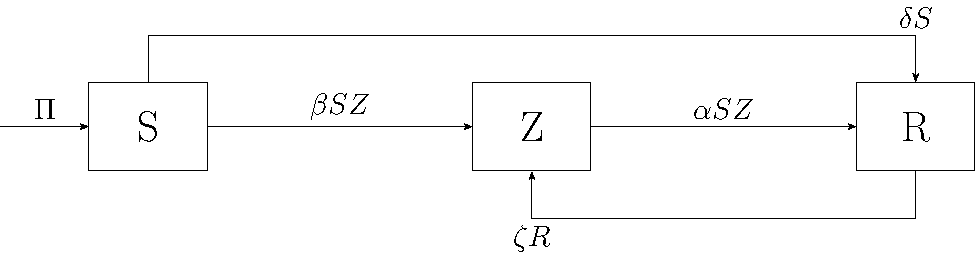
\includegraphics[width=0.9\textwidth]{SRZ.pdf}
\end{center}
Từ mô hình này, ta có thể nhìn ra được rằng $S' + Z' + R' = \Pi$ nên $S + Z + R \to +\infty$ khi $t \to +\infty$ nếu $\Pi > 0$.
Điều trên chứng tỏ ra trong ba hàm $S,R,Z$ sẽ có một vài hàm có thể tiến ra vô cùng mãi mãi. 
 
Nếu $\displaystyle\lim_{t \to +\infty}S(t) = +\infty$ thì sẽ dẫn tới $\displaystyle\lim_{t \to +\infty}( - \beta SZ - \delta S )= -\infty$, tức là $S(t)$ sẽ giảm về vô cùng, vô lý. Do đó chỉ có thể $Z$ hoặc $R$ tiến ra vô cùng, và hiển nhiên, $S$ sẽ giảm dần về $0$, tức là kịch bản nhân loại diệt vong của nhân loại sẽ xảy ra nếu ta không có biện pháp can thiệp. Từ đây ta rút ra được một kết luận quan trọng:

\begin{theorem}
    Khi đại dịch Zombie xảy ra, nếu không có biện pháp can thiệp, thì nhân loại sẽ diệt vong.
\end{theorem}

Giờ ta sẽ xét đến điểm cân bằng (Equalibrium Stability Points) trong mô hình này. Trước hết, ta nhắc lại một số định nghĩa như sau:

\begin{definition}
    Một điểm cân bằng của hệ phương trình vi phân là một điểm $(S_0, Z_0, R_0)$ sao cho $S' = 0$, $Z' = 0$, $R' = 0$ tại điểm đó.
\end{definition}
\begin{definition}
    Một điểm cân bằng là ổn định nếu mọi điểm gần nó đều tiến về nó khi $t \to +\infty$.
\end{definition}
\begin{definition}
    Một điểm cân bằng là không ổn định nếu có ít nhất một điểm gần nó mà không tiến về nó khi $t \to +\infty$.
\end{definition}
Ta có thể tưởng tượng rằng điểm cân bằng ổn định giống như điểm chạm đáy của một cái bát, nếu ta cho viên bi vào đó và lắc, viên bi sẽ luôn quay về giá trị của điểm đó. Ngược lại, nếu ta cho viên bi nằm trên một đỉnh dốc và đẩy nó ra, nó sẽ lăn đi và không bao giờ trở về điểm đó nữa.

Trở lại với mô hình, xét tại điểm cân bằng, tức là $S' = Z' = R' = 0$. Trong khoảng thời gian ngắn đó, ta cũng có thể xem rằng tỉ lệ sinh và những cái chết non-zombie là bằng không, tức là $\Pi = \delta = 0$. Khi đó, ta sẽ có hệ phương trình như sau:
\[
    \begin{aligned}
    0 &= -\beta S Z \\
    0 &= \beta S Z+ \zeta R - \alpha S Z \\
    0 &= \delta S + \alpha S Z - \zeta R.
    \end{aligned}
\]
Giải hệ này, ta sẽ được các giá trị tức thời của $S$, $Z$, $R$ tại điểm cân bằng là:
\[
    (\overline{S}, \overline{Z}, \overline{R}) \in \{(\overline{S} ,0,0),(0,\overline{Z} ,0)\}
\]
Nói cách khác, điểm cân bằng của mô hình này là khi nhân loại diệt vong hoặc tất cả Zombie đều bị tiêu diệt. Bây giờ, để biết các điểm cân bằng này có ổn định hay không, ta sẽ xét đến ma trận Jacobi của hệ phương trình này. 

Bản chất của phép biến đổi này là phi tuyến nhưng mục tiêu của ta là xem xét hành vi xung quanh điểm cân bằng, vì thế nên ta sẽ cần sử dụng đến các công cụ xấp xỉ tuyến tính.

Ta biết rằng bản chất của ma trận là một tập hợp các vector trong không gian $\bb{R}^n$ và phép nhân ma trận là một phép biến đổi tuyến tính. Vì thế ta sẽ cần sử dụng công cụ đại số tuyến tính để phân tích hành vi của hệ xung quanh điểm cân bằng. Tới đây, có lẽ trong đầu ta sẽ hiện lên hai câu hỏi: 
\begin{enumerate}
    \item Tại sao ta lại cần phải sử dụng đại số tuyến tính trong khi mô hình này là phi tuyến?
    \item Tại sao lại ta lại chọn xem xét hành vi xung quanh điểm cân bằng mà không phải một điểm bất kỳ nào khác?
\end{enumerate}

Để trả lời được hai câu hỏi này, ta sẽ cần phải hiểu rõ hơn về ma trận Jacobi. Chẳng hạn trong không gian $\bb{R}^2$, xét phép biến đổi phi tuyến $f: \bb{R}^2 \to \bb{R}^2$. Ta có thể ví dụ rằng $f\begin{bmatrix}
    x\\y 
\end{bmatrix} = \begin{bmatrix}
    x + \sin(y)\\y + \sin(x)
\end{bmatrix}$

Khi ta cho mọi điểm $(x_0,y_0) \in \bb{R}^2$ vào hàm $f$, ta sẽ nhận được một lưới đồ thị mới có hình dạng khá là méo mó so với các lưới ô vuông ban đầu. Tuy nhiên, nếu ta chỉ xét một phần lưới rất nhỏ xung quanh một điểm $(x_1,y_1)$, ta có thể thấy rằng, lưới này sẽ gần như được biến đổi tuyến tính. Và ma trận Jacobi chính là ma trận biểu diễn phép biến đổi tuyến tính tại điểm này. 
\[
    J_{\mathbf{F}}(\mathbf{x}) =
\begin{bmatrix}
\displaystyle \frac{\partial f_1}{\partial x_1} &
\displaystyle \frac{\partial f_1}{\partial x_2} &
\cdots &
\displaystyle \frac{\partial f_1}{\partial x_n} 
\\[12pt]
\displaystyle \frac{\partial f_2}{\partial x_1} &
\displaystyle \frac{\partial f_2}{\partial x_2} &
\cdots &
\displaystyle \frac{\partial f_2}{\partial x_n} 
\\[12pt]
\vdots & \vdots & \ddots & \vdots \\[6pt]
\displaystyle \frac{\partial f_m}{\partial x_1} &
\displaystyle \frac{\partial f_m}{\partial x_2} &
\cdots &
\displaystyle \frac{\partial f_m}{\partial x_n} 
\end{bmatrix}
\]

Nói cách khác, ma trận Jacobi chính là công cụ tuyến tính hóa của hệ.

Còn câu hỏi thứ hai thì sao? Tại sao lại phải là điểm có các đạo hàm bằng 0? 

Gọi $x^*$ là điểm đang xét. Xét hệ $f: \bb{R}^n \to \bb{R}^m$ khả vi tại điểm $x^*$, khi đó tồn tại ánh xạ tuyến tính $L: \bb{R}^n \to \bb{R}^m$ sao cho
\[
    \lim_{h \to 0} \frac{|| f(x^* + h) - f(x^*) - L(h)||}{||h||} = 0. 
\]
Rõ ràng $L(h)$ là một ánh xạ tuyến tính scalar của $J_f(x^*)$. Khi đó có thể viết lại 
\[
    f(x) = f(x^*) + J_f(x^*) (x - x^*) + r(x) \approx  f(x^*) + J_f(x^*) (x - x^*)
\]
với $r(x)$ là hàm xấp xỉ thỏa mãn $\displaystyle \lim_{x \to x^*} \frac{||r(x)||}{||x - x^*||} = 0$. Rõ ràng, khi ta xét điểm cân bằng (tức $x_0$) thì ta được ngay $f(x_0) = 0$. Lấy các giá trị $x$ tiệm cận với $x_0$, ta được 
\[
    f(x) \approx J_f(x_0) (x - x_0) \tag{1}
\]

Cho phương trình $(1)$ từ xấp xỉ đến tiệm cận. Xét hệ động lực ta đang có $\dot{x} = f(x)$. Đặt hàm dao động $u = x - x_0$, ta được $\dot{u} = \dot{x}$ và từ $(1)$ ta được 
\[
    \dot{u} = J_f(x_0)u
\]
Bây giờ ta sẽ tìm công thức cho hàm $u$. Đặt $J = J_f(x_0)$, và đặt $e^{Jt} = \displaystyle\sum_{i = 0}^{\infty} \frac{J^i t^i}{i!}$ là ma trận hàm mũ của ma trận $J$. 

Ta sẽ chứng minh một tính chất quan trọng như sau:
\begin{theorem}
    $J$ khả chéo, tức là tồn tại $P^{-1}$ sao cho $J = P\Lambda P^{-1}\lra$ $J$ có $n$ eigenvector độc lập tuyến tính. Trong đó $P= [v_1, v_2, \ldots, v_n]$ là ma trận có các eigenvector $v_i$ làm cột và $\Lambda = \text{diag}(\lambda_1, \lambda_2, \ldots, \lambda_n)$ là ma trận đường chéo có các eigenvalue $\lambda_i$ của $J$ làm đường chéo.
\end{theorem}
\begin{proof}
    Ta chỉ cần chứng minh chiều thuận, với mọi $i$ ta đều có 
    \[
        J v_i = \lambda_i v_i \ra JP = \Lambda P \lra J  = P\Lambda P^{-1}.
    \]
    Hoàn tất chứng minh.
\end{proof}
Giả sử rằng $J$ có $n$ eigenvector độc lập tuyến tính. Ta có $J^2 = (P\Lambda P^{-1})(P\Lambda P^{-1}) = (P\Lambda)( P^{-1}P)(\Lambda P^{-1}) = P\Lambda^2 P^{-1}$, bằng quy nạp, ta chứng minh được $J^k = P\Lambda^k P^{-1}$ với mọi $k \in \bb{N}$. Từ đây suy ra 
\[
    e^{Jt} = P e^{\Lambda t} P^{-1} 
\]
Vì $\Lambda$ là ma trận đường chéo nên bằng định nghĩa chuỗi lũy thừa như trên ta tính được 
\[
    e^{\Lambda t} = \text{diag}(e^{\lambda_1 t}, e^{\lambda_2 t}, \ldots, e^{\lambda_n t}).
\]
Ta có công thức nghiệm của $u$ là 
\[
    u(t) = e^{Jt} u(0) = P e^{\Lambda t} P^{-1} u(0) = P e^{\Lambda t} [P^{-1} u(0)]
\]
Bởi vì các eigenvector của $J$ độc lập tuyến tính nên tồn tại bộ số $(c_1,c_2,\dots,c_n) \in \bb{R}^n$ sao cho $u(0) = c_1 v_1 + c_2 v_2 + \ldots + c_n v_n$. Khi đó phép biến đổi tuyến tính $P^{-1}$ sẽ biến $u(0)$ thành một vector cột có các thành phần là các hệ số tuyến tính của các eigenvector. Tức là \[P^{-1} u(0) = \begin{bmatrix}
    c_1 \\ c_2 \\ \vdots \\ c_n
\end{bmatrix} \ra e^{\Lambda t} [P^{-1} u(0)] = \begin{bmatrix}
    c_1 \\ c_2 \\ \vdots \\ c_n
\end{bmatrix}\cdot\begin{bmatrix}
e^{\lambda_1 t} & 0 & \cdots & 0 \\
0 & e^{\lambda_2 t} & \cdots & 0 \\
\vdots & \vdots & \ddots & \vdots \\
0 & 0 & \cdots & e^{\lambda_n t}
\end{bmatrix} = \begin{bmatrix}
    c_1 e^{\lambda_1 t} \\ c_2 e^{\lambda_2 t} \\ \vdots \\ c_n e^{\lambda_n t}
\end{bmatrix} = A \]
\[
    \ra u(t) = P.A = [v_1,v_2,\ldots,v_n]\cdot \begin{bmatrix}
    c_1 e^{\lambda_1 t} \\ c_2 e^{\lambda_2 t} \\ \vdots \\ c_n e^{\lambda_n t} 
\end{bmatrix}= \sum_{i = 1}^n c_i e^{\lambda_i t} v_i
\]
Với các $\lambda_i$ là các eigenvalue của ma trận $J$, tức là nghiệm của phương trình 
\[
    \det(J - \lambda I) = 0.
\]
Từ công thức của $u(t)$, ta có thể suy ra được hành vi của hệ phương trình vi phân này. Năm 1959, hai nhà toán học người Mỹ Philip Hartman và Lev Grobman đã phát triển một định lý quan trọng về hành vi của hệ phương trình vi phân tuyến tính gần điểm cân bằng. Và trên đây ta đã chứng minh được một phần để có cái nhìn rõ ràng hơn về định lý này. Định lý được phát biểu theo dạng đơn giản như sau:
\begin{theorem}(\vocab{Định lý Hartman-Grobman})
Gần một điểm cân bằng (tức tất cả các trị riêng của ma trận Jacobian tại điểm đó đều có phần thực khác $0$), hệ phương trình phi tuyến
\[
\dot{\mathbf{x}} = \mathbf{f}(\mathbf{x})
\]
có quỹ đạo gần điểm cân bằng giống về hình dạng với quỹ đạo của hệ tuyến tính hóa
\[
\dot{\mathbf{u}} = J\mathbf{u}.
\]
Cụ thể, nếu các eigenvalue đều có các phần thực là âm, thì hệ thống ổn định gần điểm cân bằng. Nếu bất kỳ eigenvalue nào có phần thực dương, thì điểm đó không ổn định. Nếu phần thực lớn nhất của các eigenvalue bằng không, ma trận Jacobian không thể đánh giá độ ổn định.
\end{theorem}

Bây giờ nếu đã đi đến được đây thì ta đã có đủ kiến thức để hiểu về cách phân tích hành vi của hệ phương trình phi tuyến này và cả khi nó được cải tiến ở các phần sau.

Quay trở lại mô hình hệ SRZ có các phương trình vi phân như sau:
\[
    \begin{aligned}
    S' &= \Pi - \beta S Z - \delta S \\
    Z' &= \beta S Z + \zeta R - \alpha SZ\\
    R' &= \delta S + \alpha SZ - \zeta R.
    \end{aligned}
\]
có các điểm cân bằng là $(\overline{S} ,0,0),(0,\overline{Z} ,0)$ và giả sử rằng $\Pi = \delta = 0$. Jacobian của hệ tại một điểm bất kỳ là 
\[  
    J = \begin{bmatrix}
    -\beta Z  & -\beta S & 0 \\
    \beta Z - \alpha Z & \beta S - \alpha S & \zeta \\
     \alpha Z& \alpha S & -\zeta
    \end{bmatrix}
\]
Tại điểm cân bằng $(\overline{S} ,0,0)$, Jacobian của hệ sẽ là 
\[
    J(\overline{S},0,0) = \begin{bmatrix}
    0 & -\beta \overline{S} & 0 \\
    0 & \beta\overline{S} - \alpha\overline{S} & \zeta \\
    0 & \alpha\overline{S} & -\zeta
    \end{bmatrix}
\]
Ta sẽ tính eigenvalue của ma trận này bằng cách giải phương trình $\det(J - \lambda I) = 0$. Giải phương trình này ta được 
\[
\det(J-\lambda I) =
\lambda \bigg[
-\lambda^2 +
\big( (\beta-\alpha)\overline{S} - \zeta \big)\lambda +
\zeta\beta\overline{S}
\bigg]
\]
Bởi vì $-\zeta\beta\overline{S} < 0$ nên phương trình này có một nghiệm dương nên hệ này không ổn định. Tương tự, tại điểm cân bằng $(0,\overline{Z},0)$, ta cũng sẽ có ma trận Jacobian là
\[
    J(0,\overline{Z},0) = \begin{bmatrix}
    -\beta \overline{Z} & 0 & 0 \\
    \beta \overline{Z}  -\alpha \overline{Z} &0 & \zeta \\
     \alpha \overline{Z} & 0 & -\zeta
    \end{bmatrix} 
\]
Ta có $\det(J-\lambda I) = -\lambda (\lambda+\beta\overline{Z}) (\lambda+\zeta)$. Hệ này có mọi nghiệm có phần thực đều âm nên kết luận hệ ổn định.

Câu hỏi ở đây là, tại sao trong trường hợp không có Zombie nào thì về sau nhân loại vẫn sẽ diệt vong vì Zombie? Hãy nên nhớ người chết có thể hồi sinh và trở thành Zombie, và đây là một nguồn tạo ra Zombie ổn định qua thời gian. Vì thế điểm cân bằng này không bao giờ là ổn định.

Dưới đây là đồ thị trong trường hợp $\Pi = 10,
\beta = 0.0095,
\delta = 0.0001,
\zeta = 0.1,
\alpha = 0.0005, R_0 = 1, S_0 = 500$
\begin{center}
    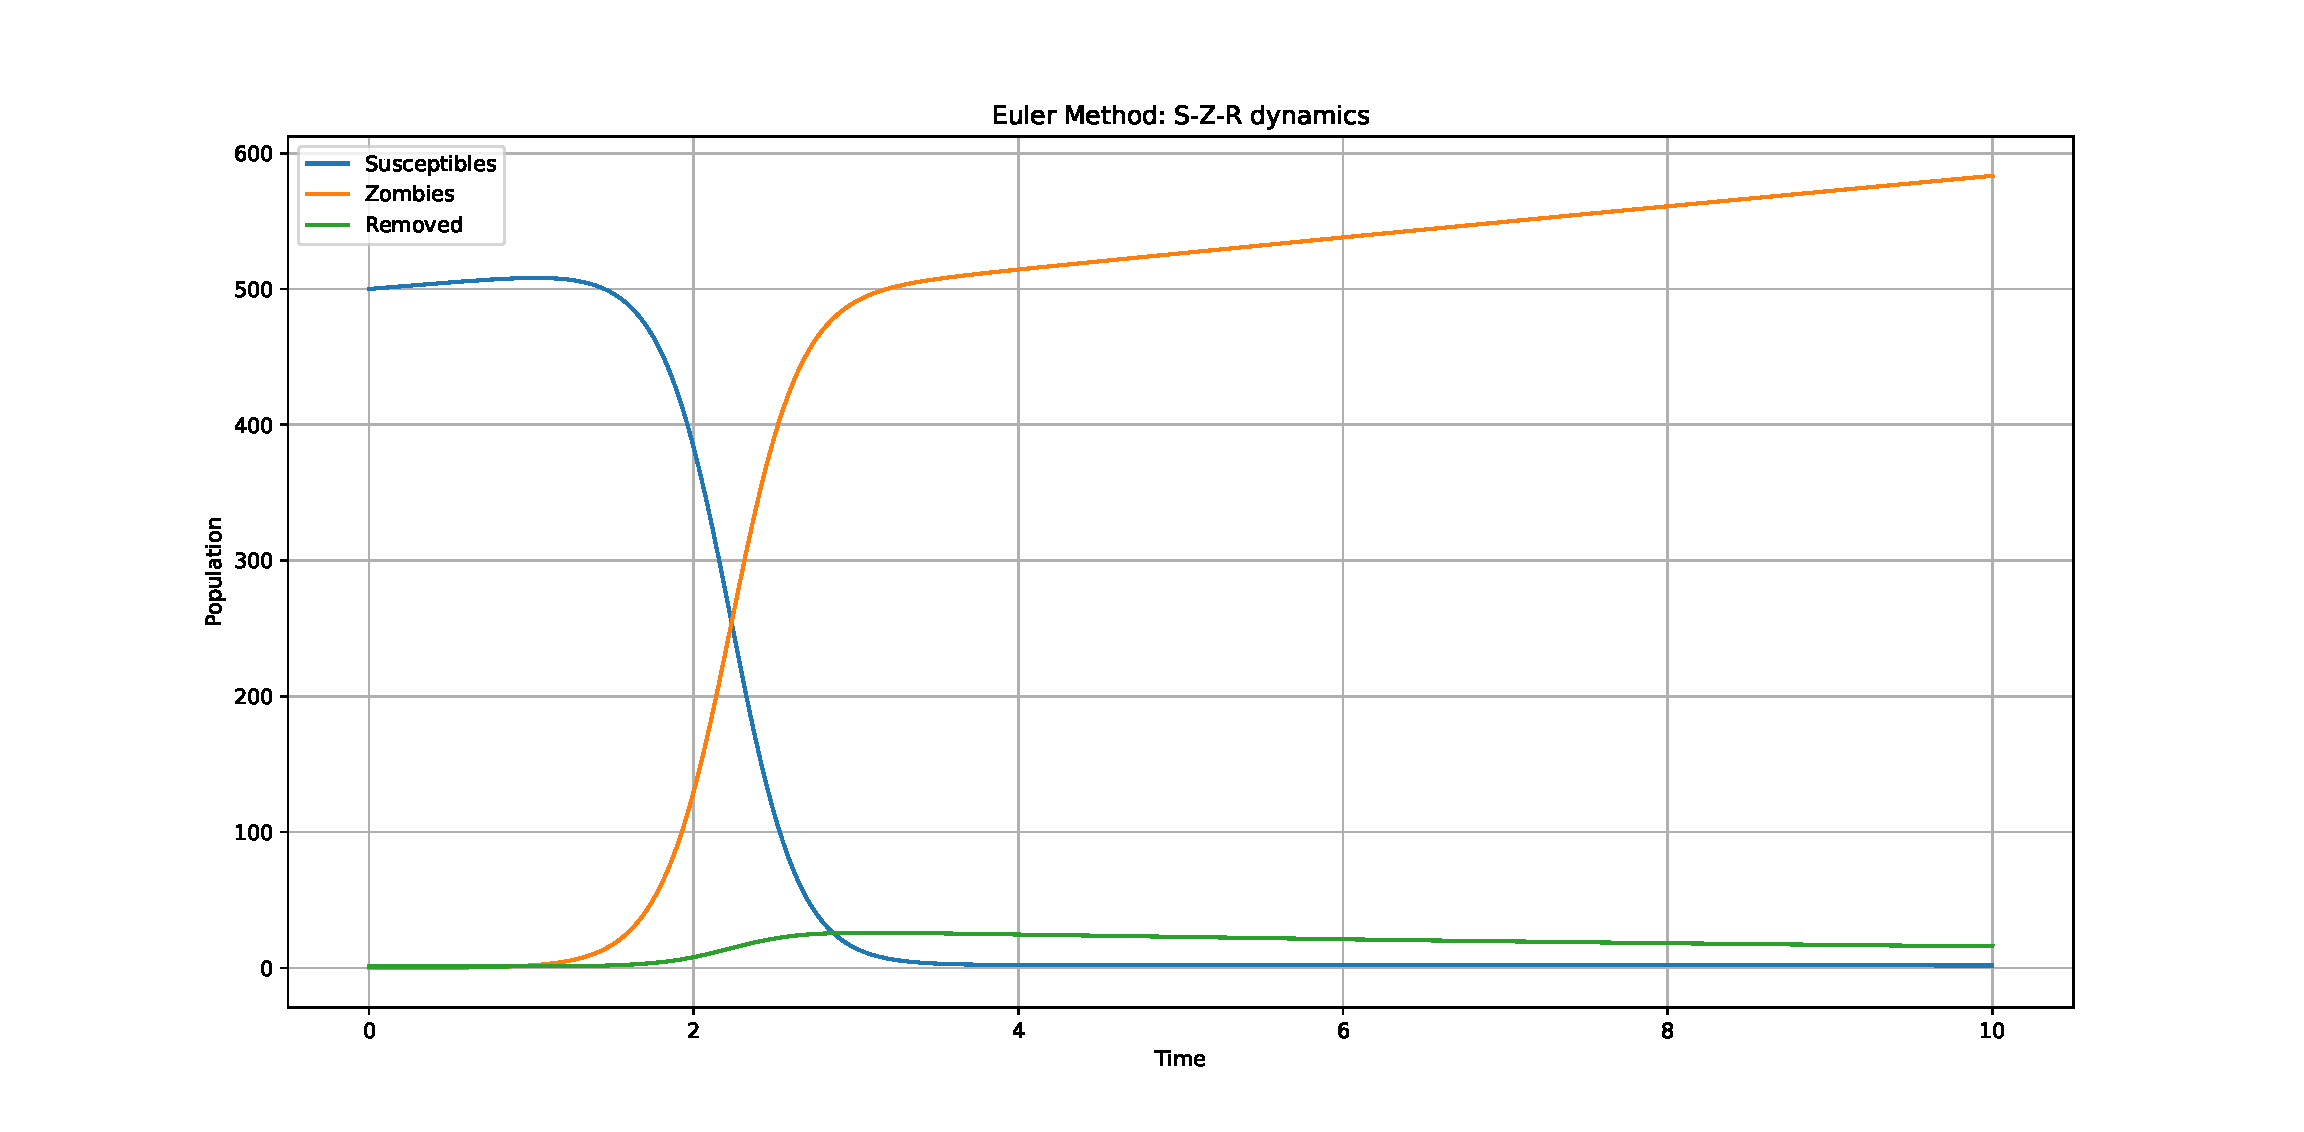
\includegraphics[width=1\textwidth]{Figure_1.pdf}
\end{center}

Trong một vài trường hợp, loài người sẽ tiêu diệt hoàn toàn Zombie và cũng có trường hợp Zombie sẽ thống trị loài người mặc dù số lượng ban đầu rất ít. Vậy thì để dự đoán rằng trường hợp nào sẽ xảy ra, ta cần một khái niệm mới - Hệ số sinh sản cơ bản, được ký hiệu là $R_0$ và được tính bằng 
\[
    R_0 = \frac{\text{Tốc độ tạo ra ca nhiễm mới}}{\text{Tốc độ thoát khỏi trạng thái lây nhiễm}} 
\]
Trong mô hình SRZ, $R_0 = \frac{\beta}{\alpha}$. 
\section{Mô hình với quá trình nhiễm trùng tiềm ẩn}
 Trong thực tế, khi một người khỏe mạnh tiếp xúc với Zombie, Virus của Zombie có thể cần một thời gian nhất định để xâm chiếm vật thể và biến chủ thể thành Zombie. Bây giờ ta sẽ nghiên cứu thêm một đối tượng liên quan là lớp bị nhiễm bệnh (Infected). Đối tượng này phải thỏa mãn hai điều kiện:
 \begin{itemize}
    \item Người khỏe mạnh (Susceptibles) phải đi qua lớp và ở đó trong một thời gian trước khi trở thành Zombie
    \item Người bị nhiễm (Infected) vẫn có thể chết một cách tự nhiên trước khi trở thành Zombie.
 \end{itemize}
Và ta cũng gọi $\rho$ là tốc độ người bị nhiễm trở thành Zombie. Khi đó ta được mô hình SIZR như sau:
\[
 \begin{aligned}
    S' &= \Pi - \beta S Z - \delta S\\
    I' &= \beta S Z - \rho I - \delta I\\
    Z' &= \rho I + \zeta R - \alpha S Z\\
    R &= \delta S + \delta I + \alpha S Z - \zeta R
 \end{aligned}
\]
Mô hình có thể được sơ đồ hóa như sau:
\begin{center}
    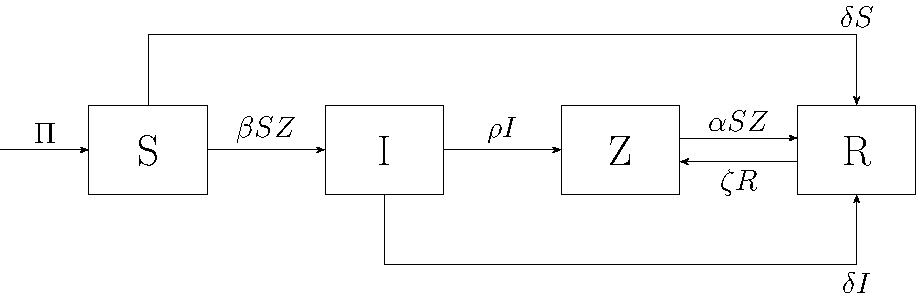
\includegraphics[width=0.9\textwidth]{SIZR.pdf}
\end{center}
Dễ thấy hai điểm cân bằng của hệ này lại là $(\overline{S},0,0,0)$ và $(0,0,\overline{Z},0)$. Vì thế con người và Zombie không thể cùng nhau tồn tại lâu dài được. Jacobian của hệ là 
\[
    J = \begin{bmatrix}
        -\beta Z & 0 & -\beta S & 0\\
        \beta Z & \rho & \beta S & 0\\
        -\alpha Z & \rho & -\alpha S & \zeta \\
        \alpha Z & 0 & \alpha S & -\zeta
    \end{bmatrix}
\]
Ta vẫn sẽ đi đánh giá giá trị của eigeinvalue của Jacobian trong từng điểm cân bằng. Đầu tiên là 
\[
    \begin{aligned}
        \det(J(\overline{S},0,0,0) - \lambda I) &=\det \begin{bmatrix}
        \lambda & 0 & \beta \overline{S} & 0\\
        0 & -\rho - \lambda & \beta \overline{S} & 0\\
        0 & \rho & -\alpha\overline{S} - \lambda & \zeta\\
        0 & 0 & \alpha \overline{S} & -\zeta - \lambda
    \end{bmatrix}\\
    & = -\lambda \det\begin{bmatrix}
        -\rho - \lambda & \beta\overline{S} & 0\\
        \rho & -\alpha\overline{S} - \lambda & \zeta\\
        0 & \alpha\overline{S} & -\zeta - \lambda
    \end{bmatrix}\\
    & = \lambda[-\lambda^3 - (\rho + \zeta + \alpha\overline{S})\lambda^2 - (\rho\alpha\overline{S} + \rho\zeta - \rho\beta\overline{S})\lambda\\
    & + \rho\zeta\beta\overline{S}]
    \end{aligned}
\]
Vì $\rho\zeta\beta\overline{S} > 0$ nên phương trình trên có 1 nghiệm dương, vì vậy điểm cân bằng này không ổn định. Tiếp theo, ta có 
\[
\det\big( J(0,0,\bar{Z},0) - \lambda I \big) =
\det \begin{bmatrix}
-\beta \bar{Z} - \lambda & 0 & 0 & 0 \\
\beta \bar{Z} & -\rho - \lambda & 0 & 0 \\
-\alpha \bar{Z} & \rho & -\lambda & \zeta \\
\alpha \bar{Z} & 0 & 0 & -\zeta - \lambda
\end{bmatrix}.
\]
Các eigeinvalue là $\lambda \in \{0,-\beta\overline{Z}, -\rho, -\zeta\}$, tất cả đều âm, chứng tỏ rằng cho dù quá trình này bị trì hoãn bởi người bị lây nhiễm cần thời gian để trở thành Zombie, về sau cùng, Zombie vẫn sẽ chiếm phần lớn dân số. $R_0$ trường hợp này vẫn là $\frac{\beta}{\alpha}$.

\section{Mô hình với yếu tố Cách ly}
Bởi vì con người không thể sống chung với Zombie, ta cần phải có biện pháp để đối phó với người mắc bệnh và Zombie, và một phương pháp tương đối hiệu quả hiện nay đó là cách ly (Quarantine). Đối tượng thuộc lớp Quarantine sẽ thỏa mãn các điều sau:
\begin{itemize}
\item Khu vực cách ly chỉ bao gồm những người bị nhiễm bệnh (Infected) và Zombie. Và những đối tượng này sẽ tăng vào khu cách ly với tốc độ lần lượt là $\kappa$ và $\sigma$.
\item Có một khả năng rằng một vài người trong khu cách ly sẽ cố gắng chạy trốn ra bên ngoài, nhưng họ đều sẽ bị giết trước khi đào thoát thành công (tỉ lệ $\gamma$).
\item Những người bị giết đó sẽ được vào lớp Removed và có thể trở thành Zombie.
\end{itemize}

Hệ SIZRQ bây giờ sẽ là 
\[
    \begin{aligned}
        S' &= \Pi - \beta SZ - \delta S\\
        I' &= \beta SZ - \rho I - \delta I - \kappa I\\
        Z' &= \rho I + \zeta R - \alpha SZ - \sigma Z \\
        R' &= \delta S + \delta I + \alpha SZ - \zeta R + \gamma Q\\
        Q &= \kappa I + \sigma Z - \gamma Q
    \end{aligned}
\]
Hệ có thể sơ đồ hóa như sau:
\begin{center}
    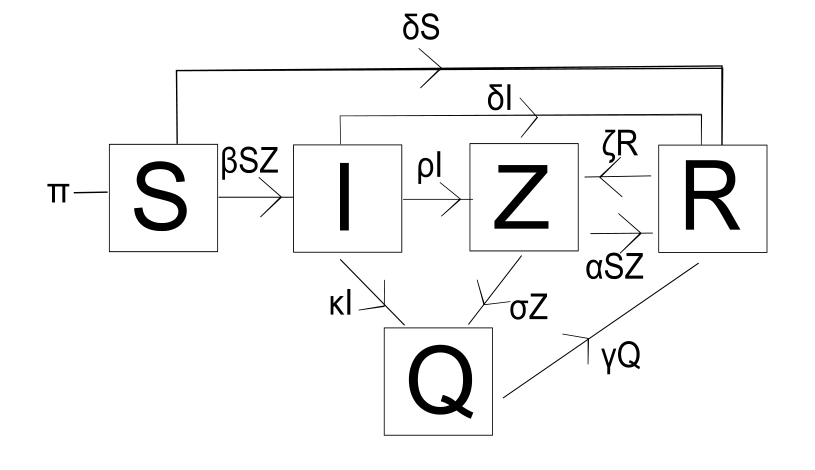
\includegraphics[width=0.8\textwidth]{SIZRQ.png}
\end{center}
Trong khoảng thời gian ngắn $(\Pi = \delta = 0)$, ta có được hai điểm cân bằng 
\[
(\overline{S},\overline{I},\overline{Z},\overline{R},\overline{Q}) = (\overline{S},0,0,0,0) = (0,0,\overline{Z},\overline{R},\overline{Q})
\]
Nếu ta tính Jacobian của hệ mà hệ chỉ cho ta kết quả là hệ ổn định hay không thì quả là phí sức khi ta cần phải tính một định thức của ma trận $5\times 5$, vì vậy ta sẽ tìm cách phân tích hành vi của hệ một cách đỡ tính toán và hiệu quả hơn. Ta sẽ quan tâm đến $R_0$ - Hệ số sinh cơ bản. Và để tìm được $R_0$, ta chỉ cần quan tâm đến ba đối tượng là $I,Z$ và $Q$. Đặt vector
\[
    u = \begin{bmatrix}
        I\\Z\\Q
    \end{bmatrix}
\]
Theo định lý Hartman-Grobman, ta có 
\[
    \dot{u}  = Ju
\]
với $J$ là Jacobian của hệ $(I',Z',Q')$. Ta tính được 
\[J = 
\begin{bmatrix}
-(\rho+\delta+\kappa) & \beta S & 0 \\[6pt]
\rho & -\alpha S - \sigma & 0 \\[6pt]
\kappa & \sigma & -\gamma
\end{bmatrix}
\]
Ta viết cách khác \[
J = \frac{\delta(\text{độ thay đổi của hệ tại }i)}{\delta x_j}\Bigg|_{x} = 
\frac{\delta(\text{độ tăng của hệ tại }i)}{\delta x_j}\Bigg|_{x} - \frac{\delta(\text{độ giảm của hệ tại }i)}{\delta x_j}\Bigg|_{x}
\]
Và ta đặt $F = 
\frac{\delta(\text{độ tăng của hệ tại }i)}{\delta x_j}\Bigg|_{x}$ và $V =\frac{\delta(\text{độ giảm của hệ tại }i)}{\delta x_j}\Bigg|_{x}$ thì có $J = F - V$, tức là có thể tìm được $F$ và $V$ bằng cách tách các số hạng hệ số của $J$. Xét sơ đồ hóa của SIZRQ, sơ đồ này mô tả độ thay đổi của từng đối tượng.
Thay điểm cân bằng $(N, 0, 0, 0, 0)$ ta tính được ma trận $F$ và $V$ có dạng như sau:
\[
F =
\begin{bmatrix}
0 & \beta.N & 0 \\[6pt]
0 & 0 & 0 \\[6pt]
0 & 0 & 0
\end{bmatrix}
,
\quad
V=
\begin{bmatrix}
    \rho+\kappa & 0 & 0 \\[6pt]
    -\rho & \alpha.N + \sigma & 0 \\[6pt]
    -\kappa & -\sigma  & \gamma
\end{bmatrix}
\]
Với $F-V = J_0$ ($J_0$ là Jacobian tại điểm cân bằng). Ta tìm ma trận nghịch đảo của $V$.
\[
V^{-1} =
\frac{1}{\gamma (\rho+\kappa)(\alpha N+\sigma)}
\begin{bmatrix}
\gamma (\alpha N+\sigma) & 0 & 0 \\[6pt]
\rho \gamma & \gamma (\rho+\kappa) & 0 \\[6pt]
\rho \sigma + \kappa (\alpha N+\sigma) & \sigma (\rho+\kappa) & (\rho+\kappa)(\alpha N+\sigma)
\end{bmatrix}
\]
Từ đó ta tìm được hằng số $R_0$ thông qua tỉ lệ của $\frac{F}{V}$ là:
\[
FV^{-1} =
\frac{1}{\gamma (\rho+\kappa)(\alpha N+\sigma)}
\begin{bmatrix}
\beta N \rho \gamma & \beta N \gamma (\rho+\kappa) & 0 \\[6pt]
0 & 0 & 0 \\[6pt]
0 & 0 & 0
\end{bmatrix}
\]
Dễ dàng tĩnh được:
\[
R_0 = \frac{\beta N \rho}{(\rho+\kappa)(\alpha N + \sigma)}.
\]
Suy ra, trạng thái cân bằng không có dịch bệnh ổn định nếu $R_0$<1. Điều này có thể làm được bằng cách tăng $\kappa$ hoặc $\sigma$ tức là tốc độ cách ly người bị nhiễm bệnh và Zombie tương ứng. Nếu quy mô quần thể lớn thì:
\[
R_0 \approx \frac{\beta \rho}{(\rho+\kappa)\alpha}.
\]
 Nếu (Zombie lây nhiễm con người nhanh hơn con người tiêu diệt Zombie, như chúng ta dự đoán), thì
 việc tiêu diệt dịch bệnh phụ thuộc rất nhiều vào việc cách ly những người ở giai đoạn đầu của quá trình
 nhiễm. Điều này có thể đặc biệt khó khăn nếu việc xác định những cá nhân như vậy không rõ ràng.
 \newline
 \\
  Tuy nhiên, chúng tôi cho rằng việc cách ly một tỷ lệ lớn các cá thể nhiễm bệnh là không thực tế do hạn chế
 về cơ sở hạ tầng. Vì vậy, chúng tôi không kỳ vọng các giá trị  hoặc  sẽ cao trong thực tế. Vì vậy kết quả mà chúng tôi nghiêng về hơn sẽ là $R_0$>1.
 \newline
 \\
 Cũng như trước, chúng tôi minh họa bằng phương pháp Euler. Các tham số giống như trong các mô hình
 trước. Chúng tôi điều chỉnh  để thỏa mãn  Kết quả được minh họa ở hình . Trong trường
 hợp này, hiệu quả của việc cách ly chỉ làm trì hoãn nhẹ thời gian dẫn đến sự diệt vong của loài người

\end{document}

 